\documentclass[11pt,a4paper]{article}

\usepackage[french]{babel}
\usepackage[utf8x]{inputenc}
\usepackage{amsmath}
\usepackage[top=3cm,bottom=2.5cm,left=2cm,right=2cm]{geometry}
\usepackage{nicefrac}
\usepackage{graphicx}

\title{Compte rendu: TP Instrumentation Avancée}
\author{Lechat Thomas -- Mathieu Gaborit}
\date{L2 SPI -- Janvier 2013}

\begin{document}
\maketitle

\section*{Introduction}

Le but de ce TP est de mettre en pratique les nouvelles notions d'instrumentation vues en cours au travers de l'acquisition et l'analyse de signaux par l'outil informatique.
Nous allons notament faire l'acquisition de données, les analyser d'un point de vu temporel ainsi que fréquentiel en
prenant en compte l'effet du filtre anti-repliement (FAR).
Enfin nous chercherons à retrouver un numéro de téléphone à partir de son empreinte sonore.

\section{Branchements}

Pendant toute la durée du TP, on utilise une carte NI-DAQ 9233 reliée au PC via un câble USB. L'acquisition et
l'enregistrement des signaux ont été réalisés \textit{via} une application LabVIEW\textsuperscript{\textregistered}.

\section{Bases}

On réalise une première acquisition correspondant à une note chantée échantillonnée à $F_e=50KHz$. Le nombre de points
est fixé à$N=50000$ afin d'avoir une durée d'acquisition de 1 seconde, la dynamique d'entrée est fixée a $\pm 5V$. 
 
On identifie les colonnes du fichier créé par LabVIEW\textsuperscript{\textregistered} lors de l'acquisition comme suit :

\begin{description}
\item[Colonne 1] temps (en s)
\item[Colonne 2] signal (en Pa)
\end{description}

Le signal est ensuite visualisé en utilisation MATLab\textsuperscript{\textregistered}.

\subsection{Vérification de la fréquence d'échantillonnage}

Pour identifier la fréquence d'échantillonnage, un \textit{zoom} sur les 5 premiers points du signal est réalisé. On remarque qu'entre 2 points, on a une durée de $2 \cdot 10^{-5}s$.
C'est notre période d'échantillonnage $T_e$. On a $F_e = \nicefrac{1}{Te}$, donc $F_e = 50000 Hz$. La fréquence qu'on
trouve via le logiciel MATLab\textsuperscript{\textregistered} est donc bien celle paramètrée dans LabVIEW\textsuperscript{\textregistered}.

De plus, lors d'une analyse fréquentielle, la documentation technique de la carte stipule que, dans le cas où la
fréquence d'échantillonnage est inférieure à $25 600kS/s$\footnote{\textit{kilosample per second}}, le signal est filtré
à partir de $0.42F_e$ afin d'eviter les phénomènes de repliement (le FAR coupe à $0.32fe$ dans le cas d'une fréquence
supérieure a $25 600kS/s$.


\subsection{Calcul du pas de quantification}

On cherche maintenant à determiner le pas de quantification qui à été utilisé lors de l'acquisition.

On a $\Delta V=5V$, $N = 24 bits$ :

\begin{eqnarray*}
dV & = & \frac{2*\Delta V}{2^N} \\
   & = &  \frac{10}{2^{24}} \\
dv & \approx & 59,6 \cdot 10^{-7} V
\end{eqnarray*}

Celui-ci est donc extrêmement petit.
Avec une carte d'acquisition 24bits, il est donc impossible de retrouver le pas de quantification de manière graphique étant donné son ordre de grandeur.

L'erreur commise lors de léchantillonnage est donc négligeable : le pas de quantification est donc extrêmement faible
comparativement aux mesures effectuées ainsi qu'au bruit ambiant de la salle.

\section{Analyse Spectrale}


La fréquence fondamentale de la note émise par Thomas (notre chanteur du jour) est de $F_0=1013Hz$.

\subsection{Détermination de la précision fréquentielle}

On regarde, sur le graphe, l'écart fréquentiel entre 2 points consécutifs. On trouve : $\Delta f_{obs} = 1Hz$.

On a $F_e = 50kHz$, $N = 50000$ et donc :

$$\Delta f_{th} = \frac{Fe}{N} = 1Hz$$

Ce résultat correspond à nos observations sur le graphe.

Notre erreur sur la mesure est donc d'environ $df = 0,5Hz$, d'où :

$$F_0 = 1013\pm 0,5 Hz$$


En divisant par quatre la durée d'acquisition, on divise par quatre le nombre de points et la précision fréquentielle $df$ ; sachant que :

$$df  = \frac{F_e}{2N} = \frac{\Delta f}{2}$$

On a donc $df$ quatre fois plus grand avec 0.25s d'acquisition qu'avec 1s, on commet par conséquent une erreur quatre fois plus grande.

\subsection{Effet du FAR}

Le schéma en figure~\ref{FAR} représente la coupure d'un FAR sur un spectre : on remarque que le pic lié à la
périodisation et aux replis (après $\nicefrac{F_e}{2}$) est coupé par le FAR.

\begin{figure}[h!]
\begin{verbatim}
A                0.42Fe (parce qu'on est en dessous de 25.56kS/s)
+-------------------+
|                    \ Coupure du FAR
|                     \                      
|                |     \         |            
|                |      \        |            
|                |       \       |            
|                |        \      |            
+----------------+-------+-------+-----------------+---->f
                        Fe/2                       Fe
\end{verbatim}
\caption{\label{FAR}Coupure d'un FAR}
\end{figure}

Dans un cas hypothétique où le FAR serait désactivé, si de l'information existe au dessus de $\nicefrac{F_e}{2}$, alors, des pics apparaîtront en dessous
de $\nicefrac{F_e}{2}$ mais ceux ci sont fictifs (dus au repliement).

\subsection{Modélisation d'un couplage AC}

En retirant la moyenne, on modélise un couplage AC. Sur le spectre, cela supprime simplement le pic en 0Hz.

L'intérêt est que le pic en 0Hz est rarement utile (du moins pas en L2), et que celui-ci provoque un "tassement" du
graphe le rendant difficilement exploitable.

\section{Niveau Sonore}

On s'interesse maintenant au calcul du niveau sonore pleine bande résultant d'une acquisition.

Le son sur lequel nous travaillons est celui de Thomas soufflant dans le microphone (une sorte de simulation de bruit
large bande).

On calcule la valeur efficace du signal avec la formule:

\begin{equation}
P_{RMS} = \sqrt{ \frac {1}{N} \sum_{i=1}^N x_i(t)^2} 
\end{equation}
    
La pression trouvée est de $16.51Pa$.

On mesure ensuite la sensisbilité du microphone. On obtient une valeur efficace (en volts, pour un sinus de 1kHz à 1Pa) : $s = 44.1mV/Pa$.

On utilise ensuite la formule suivante pour determiner le niveau sonore pleine bande:
	\begin{equation}
    L(dB SPL) = 20 \log\left(\frac{P_{RMS}}{P_{atmo}}\right)
    \end{equation}

On obtient donc un niveau sonore pleine bande de $109dB SPL$ (en considérant un bruit blanc, non filtré).

\section{Bandes d'Octave}

Le code source pour cette partie est donnée en annexe~\ref{bandes}.
Celui-ci est commenté et répond aux questions 1 à 8.

La sortie du script nous informe sur les différentes valeurs demandées :

\begin{verbatim}
Energie : 28.7206 J
Valeur efficace : 5.3592 Pa
Niveau (bandes) : 108.5613 dB SPL
Niveau (normal) : 109.3091 dB SPL
\end{verbatim}

Le niveau retrouvé est donc cohérent avec la mesure trouvée à l'exercice précédent.

L'écart entre la mesure en spectre en bandes fines ou le spectre en bandes d'octave vient probablement du faible nombre de bandes utilisé. Un plus grand nombre de bande aurait conduit à une meilleur approche du spectre en bandes fines et le niveau aurait été plus proche.

A noter toutefois qu'un écart de $1 dB SPL$ est assez faible et reste acceptable pour un TP comme celui-ci.

Enfin, l'algorithme utilisé est légèrement différent de celui proposé. On ajoute les différents vecteurs de chaque bande dans un vecteur global que l'on trace ensuite. Le résultat est le même.

Les tracés superposés du spectre en bandes d'octaves et en bandes fines sont donnés en figure~\ref{traces}. On remarque
que les formes de l'un et l'autres sont semblables.

\begin{figure}[h!]
    \centering{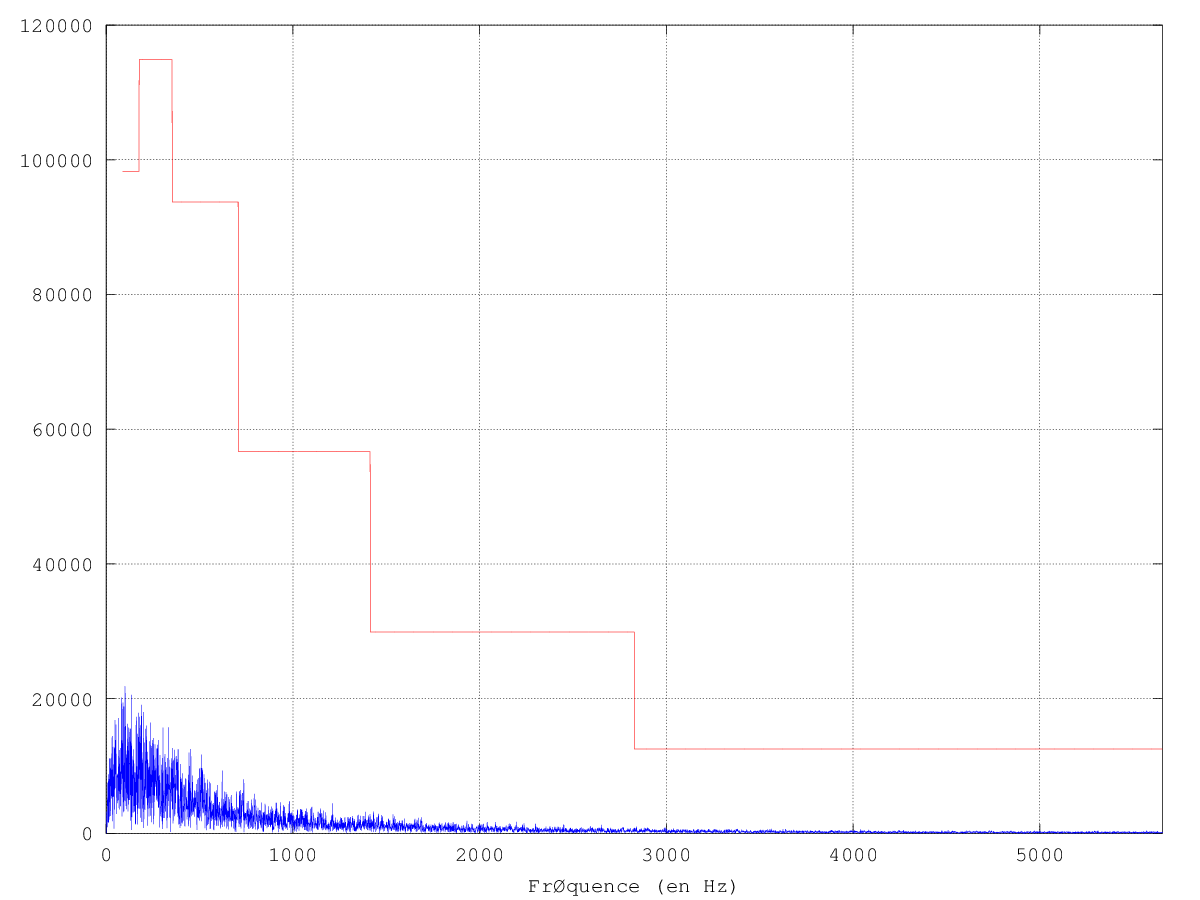
\includegraphics[width=12cm]{prog2.png}}
    \caption{\label{traces}Tracés superposés des spectres en bandes d'octaves (en rouge) et en bandes fines (en bleu)}
\end{figure}

\section{Analyse Vocale}

Un numéro est enregistré : 06 25 92 33 45.

Le découpage est ensuite fait à la main à partir du tracé temporel du signal (en fait du tracé en fonction des points,
mais c'est plus ou moins la même chose). On obtient le tableau suivant :

\begin{center}
\begin{tabular}{c||c|c}
Impulsion & Début ($\times 10^3$) & Fin ($\times 10^3$)\\\hline
1 & 0.001 & 20\\
2 & 20 & 32\\
3 & 109 & 122\\
4 & 128 & 140\\
5 & 159 & 169\\
6 & 176 & 186\\
7 & 186 & 204\\
8 & 204 & 219\\
9 & 219 & 233\\
10 & 233 & 246
\end{tabular}
\end{center}

Ce tableau est utilisé dans le script en annexe~\ref{DTFM} (variable \texttt{imps}).

D'après les informations fournies par le script (dont la sortie est reportée ci-dessous), on peut retrouver les
différents numéros à partir des couples de fréquences :

\newpage % MISE EN PAGE

\begin{verbatim}
imp #1 : 941
imp #1 : 1336
imp #2 : 770
imp #2 : 1477
imp #3 : 697
imp #3 : 1336
imp #4 : 770
imp #4 : 1336
imp #5 : 852
imp #5 : 1477
imp #6 : 697
imp #6 : 1336
imp #7 : 697
imp #7 : 1477
imp #8 : 697
imp #8 : 1477
imp #9 : 770
imp #9 : 1209
imp #10 : 770
imp #10 : 1336
\end{verbatim}

On retrouve les différents numéros :

\begin{center}
\begin{tabular}{c|c|c|c}
Num. Impulsion & Frequence 1 (Hz) & Fréquence 2 (Hz) & Numéro Correspondant\\\hline
1 & 941 & 1336 & 0\\
2 & 770 & 1477 & 6\\\hline
3 & 697 & 1336 & 2\\
4 & 770 & 1336 & 5\\\hline
5 & 852 & 1477 & 9\\
6 & 697 & 1336 & 2\\\hline
7 & 697 & 1477 & 3\\
8 & 697 & 1477 & 3\\\hline
9 & 770 & 1209 & 4\\
10 & 770 & 1336 & 5
\end{tabular}
\end{center}

Cette méthode de reconnaissance est simple et est réalisable "à l'oreille". C'est d'ailleurs pour ça qu'elle n'est plus
considérée sûre dans les dispositifs d'accessibilité pour mal-voyants (notament au niveau des distributeur bancaires).

\section*{Conclusion}

En conclusion ce TP nous aura permis de mieux cerner les notions vues en cours au travers de nos premières acquisitions sur ordinateur. Nous avons de plus pu mieux prendre en main MATLab\textsuperscript{\textregistered} et apprendre à générer de nouveau graphes (spectre en bandes d'octave, etc...).

La dernière partie (reconnaissance DTFM) a permis d'appliquer nos connaissances à un problème concret et de comprendre pourquoi cette méthode n'était pas sécurisée.

\newpage

\appendix
\begin{center}\Huge{Annexes}
\end{center}

\section{Programme pour le spectre en bandes d'octave}
\label{bandes}

\begin{verbatim}
clear all;
close all;

Fe = 50000;
Ntfd = 50000;
df = Fe/Ntfd;

freqs_centre = [0.125 0.25 0.5 1 2 4];
freqs_centre = freqs_centre*1000; % passage en kHz

freqs_inf = freqs_centre/sqrt(2);
freqs_sup = freqs_centre*sqrt(2);

file = load('bb2.lvm');

t = file(:,1);
x = file(:,2);
x = x-mean(x);

% y désigne le spectre
y = fft(x);

% axe des fréquences
freqs = (0:(length(x)-1))*(Fe/length(x));

% boucle de calcul
i = 1;
bandes = [];
energie = 0;
while i<=length(freqs_centre)

	% on récupère les indices de début et de fin
    % sur les fréquences
    ind_min = max(find(freqs <= freqs_inf(i)));
    ind_max = max(find(freqs <= freqs_sup(i)));
    
    % on extrait la séquence à analyser
    yi = y(ind_min:ind_max);
	
    % calcul de l'amplitude
	Ayi = sqrt(sum(abs(yi).^2));
    
    % longueur de la bande
    Ni = length(yi)-1;
    
    % on recrée le vecteur qui va bien
    vectAyi = Ayi*ones(1,Ni);
    
    % on l'ajoute au reste des vecteurs de bandes
    bandes = [bandes vectAyi];
    
    % energie (pour ajout à l'energie totale)
    energie = energie+Ayi^2;
    i = i+1;
end

% petit hack pour ne pas compter deux fois, 
% mais éviter les calculs inutiles
bandes = [bandes Ayi];

% Energie
energie = (energie/(Ntfd^2))*2;
eff = sqrt(energie);
disp(['Energie : ' num2str(energie) ' J']);
disp(['Valeur efficace : ' num2str(eff) ' Pa']);
lvl_b = 20*log10(eff/2e-5);
lvl_n = 20*log10(std(x)/2e-5);
disp(['Niveau (bandes) : ' num2str(lvl_b) ' dB SPL']);
disp(['Niveau (normal) : ' num2str(lvl_n) ' dB SPL']);

freqs_b = (min(freqs_inf):df:max(freqs_sup));
 
plot(freqs_b, bandes, 'r');
hold on;
plot(freqs, abs(y));
grid on;
xlim([0 max(freqs_sup)]);

\end{verbatim}

\section{Programme pour la reconnaissance des touches}
\label{DTFM}

\begin{verbatim}
clear all;
close all;

% globales
Fe = 50000;
Ntfd = 50000;


% Début et fin des impulsions
% répérés à la main
% On prends les valeurs en points/1000
imps = [
    1e-3 20;
    20 32;
    109 122;
    128 140;
    159 169;
    176 186;
    186 204;
    204 219;
    219 233;
    233 246
    ];

% on repasse aux valeurs "normales" (sans le /1000)
imps = imps*1000;

% On charge le fichier de mesures
file = load('num1.lvm');
signal = file(:,2);

% couplage AC
signal = signal - mean(signal);


% Axes des fréquences
freqs = (0:Ntfd-1)*(Fe/Ntfd);


% Boucle de reconnaissance
i = 1;
while i<=length(imps)

	% on isole la séquence intéressante
    seq = signal(imps(i,1):imps(i,2));
    
    % on calcule |FFT(sequence)|
    spk = abs(fft(seq, Ntfd));
    
    % pour DEBUG
    % plot(freqs, spk);
    
    % voir explication en dessous du code    
    % first one
    [maxi, maxi_id] = max(spk(500:1000));
    disp(['imp #' num2str(i) ' : ' num2str(freqs(maxi_id+499))]);
    
    % second one
    [maxi, maxi_id] = max(spk(1000:2000));
    disp(['imp #' num2str(i) ' : ' num2str(freqs(maxi_id+999))]);
    
    % passage à l'impulsion suivante
    i = i+1;
end
\end{verbatim}

Pour la dernière partie de la boucle : on sait que nos impulsions sont dans les bandes $[500,1000]Hz$ et $[1000;2000]Hz$. On découpe donc notre spectre en deux parties et on recherche l'indice du maximum dans cette bande. On affiche ensuite la fréquence correspondante (en reportant cette indice sur l'axe des fréquences).

\end{document}
